One reason that industrial practitioners and academics believe so strongly in the delayed issue effect is that it is often referenced
in the SE literature. For example,
we know that \fig{b81} has been presented to the gradaute SE class at North Carolina State University, without quarrel or critical comment, every year for the last decade.

Yet when we look at the literature, the evidence for
delayed issue effect is both very sparse and very old.
The first data on the difficulties of resolving delayed issues as a function of lifecycle phase date back to large systems in the late 70s from IBM~\cite{Fagan76}, TRW~\cite{Boehm76}, GTE~\cite{Daly77}, and Bell Labs~\cite{Stephenson76} (Figure~\ref{fig:cost-to-fix}). These studies are most often cited by secondary sources regarding the delayed issue effect. We note that it is unclear from the text in ~\cite{Daly77} and \cite{Boehm76} if cost is defined in terms of effort, or in actual cost (i.e., labor, materiel, travel, etc).

These studies suggest that the difficulty (in terms of effort) to find and fix an error monotonically increases with lifecycle phase.  In 1990, Boehm~\cite{Boehm80} provides data suggesting that the cost-to-fix curve for small projects (from two student projects of 2000 deliverable source instructions) is flatter than for large projects (the dashed line of Figure~\ref{fig:cost-to-fix}).

\begin{figure}[!b]
 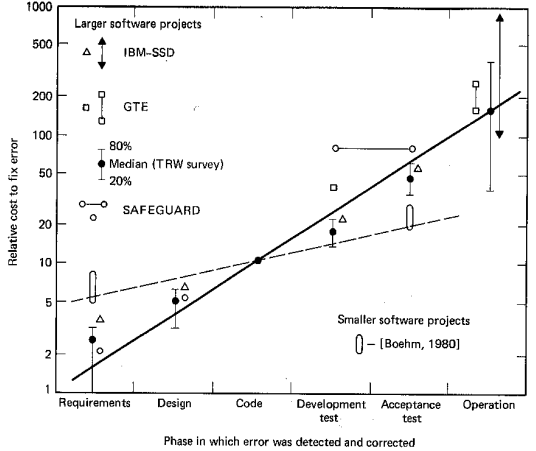
\includegraphics[width=3.3in]{img/boehm_cost-to-fix.png}
 \caption{Historical cost-to-fix curve. From~\cite{Boehm81}.}\label{fig:cost-to-fix}
 \end{figure}
 
In the 40 years since these initial studies, few studies have explored the difficulty to resolve issues
as a function of lifecycle phase. 
Shull et al.~\cite{Shull02} conducted a literature survey and held a series of e-workshops with industry experts on fighting defects. Workshop participants from Toshiba and IBM reported cost-to-fix ratios between early lifecycle and post-delivery defects of 1:137 and 1:117 for large projects respectively~\cite{Shull02} -- but we note here that the raw data points were not provided (which makes confirming those numbers 
a difficult task). 

This was a common theme in the literature reviewed for this paper-- i.e.  that  it was no longer possible to access
the data used to make prior conclusions.
As an example of this, \fig{steck} shows one 2004 survey that reports an 
exponential delayed issue  effect for 
requirements issues in eight case studies. Note that we cannot verify
{\em any} of those results since the links in the references of
that  survey are all broken (``page not found'' errors).


As to the research into agile methods, one goal of that approach
is to reduce the difficulty associated with making changes later in the lifecycle~\cite{beck00}. Relatively little empirical data exists on this point.Elssamadisy and Schalliol~\cite{Elssamadisy02} anecdotally report on the growing, high cost of rework in a 50 person, three-year, 500KLOEC Extreme Programming project as the project grew in size and complexity-- but again we cannot access their 
exact figures.


 
% We note that previous work focuses on cost-to-fix as a function of lifecycle phase irrespective of when the defect was injected, that is, previous work analyzes the cost to fix a defect found in test regardless of whether that defect was a requirements error or a coding mistake. To our knowledge, our research represents the first large-scale study of phase delay.


 \begin{figure}
{\small
\begin{center}
\begin{tabular}{r|rrrr}
 case& \multicolumn{4}{c}{Phase Requirements Issue Found }  \\
 study               &Requirements & Design & Code&  Test\\\hline
1& 1 &3& 5& 37\\  
2& 1  &    & 10 & 40 \\ 
3& 1   &    & 10 &  40 \\
4&  1  &   5 &      & 50  \\
5&  1 &3& 7& 51 \\
6& 1& 5 &33 &75  \\
7&  1 & 20 & 45 & 250 \\  
\end{tabular}
\end{center}}
\caption{Cost to resolve requirements issues, relative to resolving  during requirements. From ~\cite{steck04}.}\label{fig:steck}
\end{figure}


\begin{figure}[!t]
 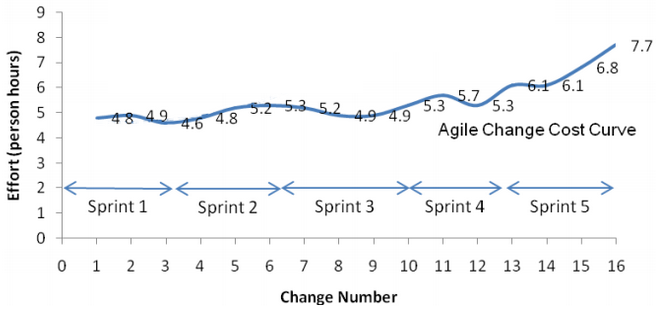
\includegraphics[width=3in]{img/clutterbuck.png} 
 \caption{Cost of change from an agile case study. From~\cite{Clutterbuck09}.}\label{fig:clutterbuck}
 \end{figure}

 
 
 All in all, the empirical results of this section seem insufficient to justify
 the strength of the beliefs documented in the previous section. Adding to our doubts are  several studies that report less-than exponential
 increase in the difficulties associated with making the changes associated with delayed
 issues. 
Clutterbuck et al.~\cite{Clutterbuck09} studied a 5-month effort by a small-to-medium enterprise team developing a 71KLOEC web interface to a database application to implement 18 change requests-- see Figure~\ref{fig:clutterbuck} (note that these were for new and changed user requirements, not defects). Clutterbuck et al. found the cost of change to be relatively flat until the later phases, with much of the effort spent in analysis of the change requests~\cite{Clutterbuck09}. Note that in this study, the effort increased by only 60\% (see the start and end of the curve in Figure~\ref{fig:clutterbuck}).




 
Another example of less-than exponential explosion in the difficulty associated with delayed issues comes from  Royce~\cite{Royce98}. He
studied  a million-line, safety-critical missile defense system
(see  Figure~\ref{fig:royce}). Design changes (including architecture changes) required approximately twice the effort of implementation and test changes, and the cost-to-fix in implementation and test phases increased slowly. Boehm~\cite{Boehm10} attributes this success to the  development process, which focused on removing architecture risk early in the development lifecycle.
 
 Other examples that report the opposite of DIE are:
  \bi
  \item
  Boehm~\cite{Boehm80} reported a flatter growth rate for small, non-critical projects.
   \item 
  Data from NASA's Johnson Space Flight Center, reported by Shull~\cite{Shull02}, found that the cost to find certain non-critical classes of defects was fairly constant across lifecycle phases (1.2 hours on average early in the project, versus 1.5 hours late in the project). 
   
\ei


\begin{figure}
 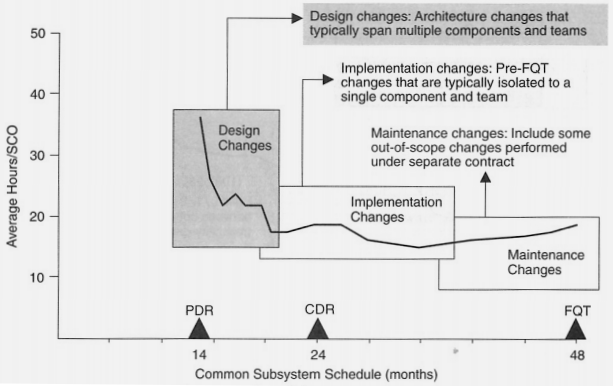
\includegraphics[width=3.3in]{img/Royce98.png}
 \caption{Exception to the rule - The Royce study: cost-to-fix curve. From~\cite{Royce98}.}\label{fig:royce}
 \end{figure}